%
%
%

\chapter{Translational Dynamical Systems}

\section{Problem Statement and Learning Objectives}
Be able to
\begin{itemize}
  \item Name system elements and write and graph constitutive relations for the basic elements
  of a translational mechanical system.
  \item Write the Equations of Motion for a translational system with any number of masses, springs, and dampers.
  \item Convert from Equations of Motion to a Transfer Function
\end{itemize}

\section{System Elements}

Translation refers to motion in a straight line.   We will first consider systems which only contains elements moving along a single direction.  Sometimes it is useful to think of this direction as a set of different but parallel axes, but this distinction does not change the physics. We only consider such systems which operate in an inertial frame such as the surface of the earth (to a good approximation at least) or inside
a vehicle moving at constant speed and direction.

% We will view the system as consisting of two types of elements:  ``active" and ``passive".  The passive elements can store or dissipate energy but cannot generate any.   The active

We will analyze systems consisting of
\begin{itemize}
  \item {\bf Mass}        The property of matter which resists acceleration, is acted on by gravity, and which stores kinetic energy.
  \item {\bf Stiffness}   The property of matter which resists displacement, and which stores potential energy.
  \item {\bf Damping}     The property of matter or interactions of matter which converts motion to heat.
\end{itemize}

Some properties of the various elements are summarized in Table \ref{TransElementsTable}.

% \setlength\extrarowheight{0.75in}
\begin{table}
\begin{tabular}{|l|l|l|l|p{2.0in}|} \hline
 Name             &  Physical Realization     &   Symbol    &  Equation              & Units and Notes   \\ \hline
  Inertia         &  Point Mass               &   $M$ \raisebox{-\totalheight}{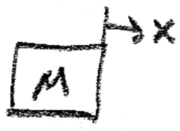
\includegraphics[width=0.6in]{figs02/00728aa.png}}     &  $f(t) = M\ddot{x}$    & $kg$, $\ddot{x}$ is with respect to the inertial frame.  \\ \hline
  Stiffness       &  Massless Spring          &   $B$ \raisebox{-\totalheight}{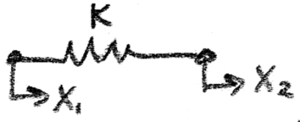
\includegraphics[width=1.0in]{figs02/00728ba.png}}    &  $f(t) = K{x}$         & $N\;m^{-1}$, $f$ is same on both sides.  Assume zero rest length \\ \hline
  Damping         &  Shock Absorber           &   $K$ \raisebox{-\totalheight}{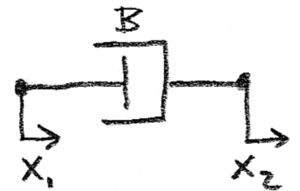
\includegraphics[width=1.0in]{figs02/00728ca.png}}   &  $f(t) = B\dot{x}$     & $N\;sec^{-1}\;m^{-1}$, This is a linear model for friction.     \\ \hline
\end{tabular}\caption{}\label{TransElementsTable}
\end{table}


\subsection{Displacements and Derivatives}

We shall analyze the state and the motion of translational systems in terms of

Position, $x(t)$, Velocity, $\dot{x}(t)$, and Acceleration, $\ddot{x}(t)$.
Where each dot represents a time derivative:
\[
\dot{x} = \frac{d}{dt}x(t) \qquad \ddot{x} = \frac{d^2}{dt^2}x(t)
\]

Often we will omit the time dependence, i.e. $\dot{x} = \dot{x}(t)$.



\subsection{Forces}

Each system element generates forces according to well known physical laws:

\begin{itemize}
  \item Mass:  $F=m\ddot{x}$.
  \item Stiffness:  $F= K(x_2-x_1)$
  \item Damping:    $F= B(\dot{x}_2- \dot{x}_1)$
\end{itemize}

In the case of stiffness and damping, the force is generated by the {\it difference} of two displacements or velocities.   In the case of Mass undergoing translational motion in an inertial frame, the force is generated only by accelerations with respect to the inertial frame.   An inertial frame is one which is not accelerating.


\subsection{Mechanical Network Schematic Diagram}

We must usually simplify the mechanical system into a purely translational one to apply the analyis of this chapter.   To do so, we identify the mass for each moving part and draw it as a box labeled $M_i$ (Figure \ref{masses}).   What each box actually represents is a point mass.  Each point mass has a displacement, $x_i$ which indicates its location along the axis of linear motion.



\begin{figure}\centering
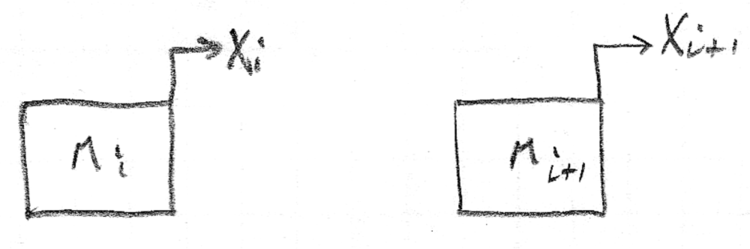
\includegraphics[width=2.5in]{figs02/00720a.png}
\caption{Each mass has an associated displacement.}\label{masses}
\end{figure}


Springs and dampers are then connected between the moving parts.   Alternatively, one end of a spring or damper may be connected to ground (a point at which $x = \dot{x} = \ddot{x} = 0$).

\begin{Example}\label{ExampleCarSuspension}

Convert the tire, wheel, and suspension elements of a typical car to a linear mass-spring-damper model.


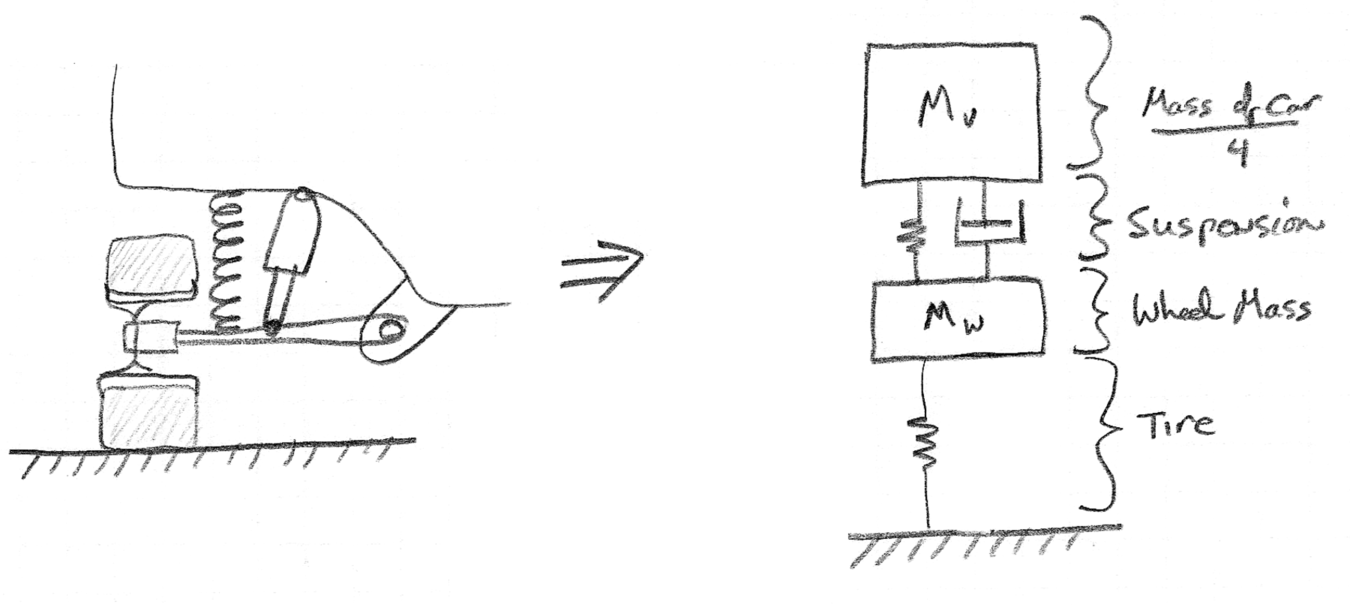
\includegraphics[width=4.5in]{figs02/00719a.png}


In this conversion we have used lots of knowledge about cars including the following facts:


 \begin{itemize}
   \item Tires are elastic and filled with a low mass material (air) and thus could plausibly be approximated by a spring.
   \item The weight of the wheel and tire can be combined into a mass.
   \item The suspension spring goes between the suspension beam and the car's body.
   \item Cars have four wheels so the mass of the body should be approximated by 1/4 of the car's total mass.
   \item The shock absorber is a damper which connects between the suspension arm and the car body (in parallel with the spring)
   \item The suspension arm is long enough compared to the tire's motion such that we can approximate the tire's motion as a straight vertical line.
 \end{itemize}


None of this knowlege is required to excel at control systems design with one exception, {\it The control system designer must have enough knowlege of the application system or access to enough model validation data to make sure that the simplified model is good enough for all application requirements. } To the extent that these ``facts" are true, our model is accurate, and to the extent that this model is an oversimplification, our model will not work.


\begin{quotation}``It can scarcely be denied that the supreme goal of all theory is to make the irreducible basic elements as simple and as few as possible without having to surrender the adequate representation of a single datum of experience." \\
{\it Albert Einstein}
\end{quotation}

\end{Example}


\section{Constitutive Relations}
Constitutive Relations are basic equations that define our system components by relating one variable to another.  For example,
a resistor relates voltage to current by Ohm's Law, $V=IR$ or a damper relates force to velocity, $F=B\dot{x}$.   Using the
analogy between force and voltage, and velocity to current, we can classify variables as ``through" or ``across" types.  Specifically

\vspace{0.25in}
\begin{tabular}{l|c|l}
           & through & across\\ \hline
Electric   & current  & voltage \\
Translation & velocity & force \\
Rotation   & angular vel.  & torque
\end{tabular}

Constitutive Relations are conventionally famous linear  functions such as
 \[
 V=IR, \; F= B\\dot{x},\; F=M\ddot{x}, \quad \mathrm{etc.}
 \]
as such they are always the same graph!

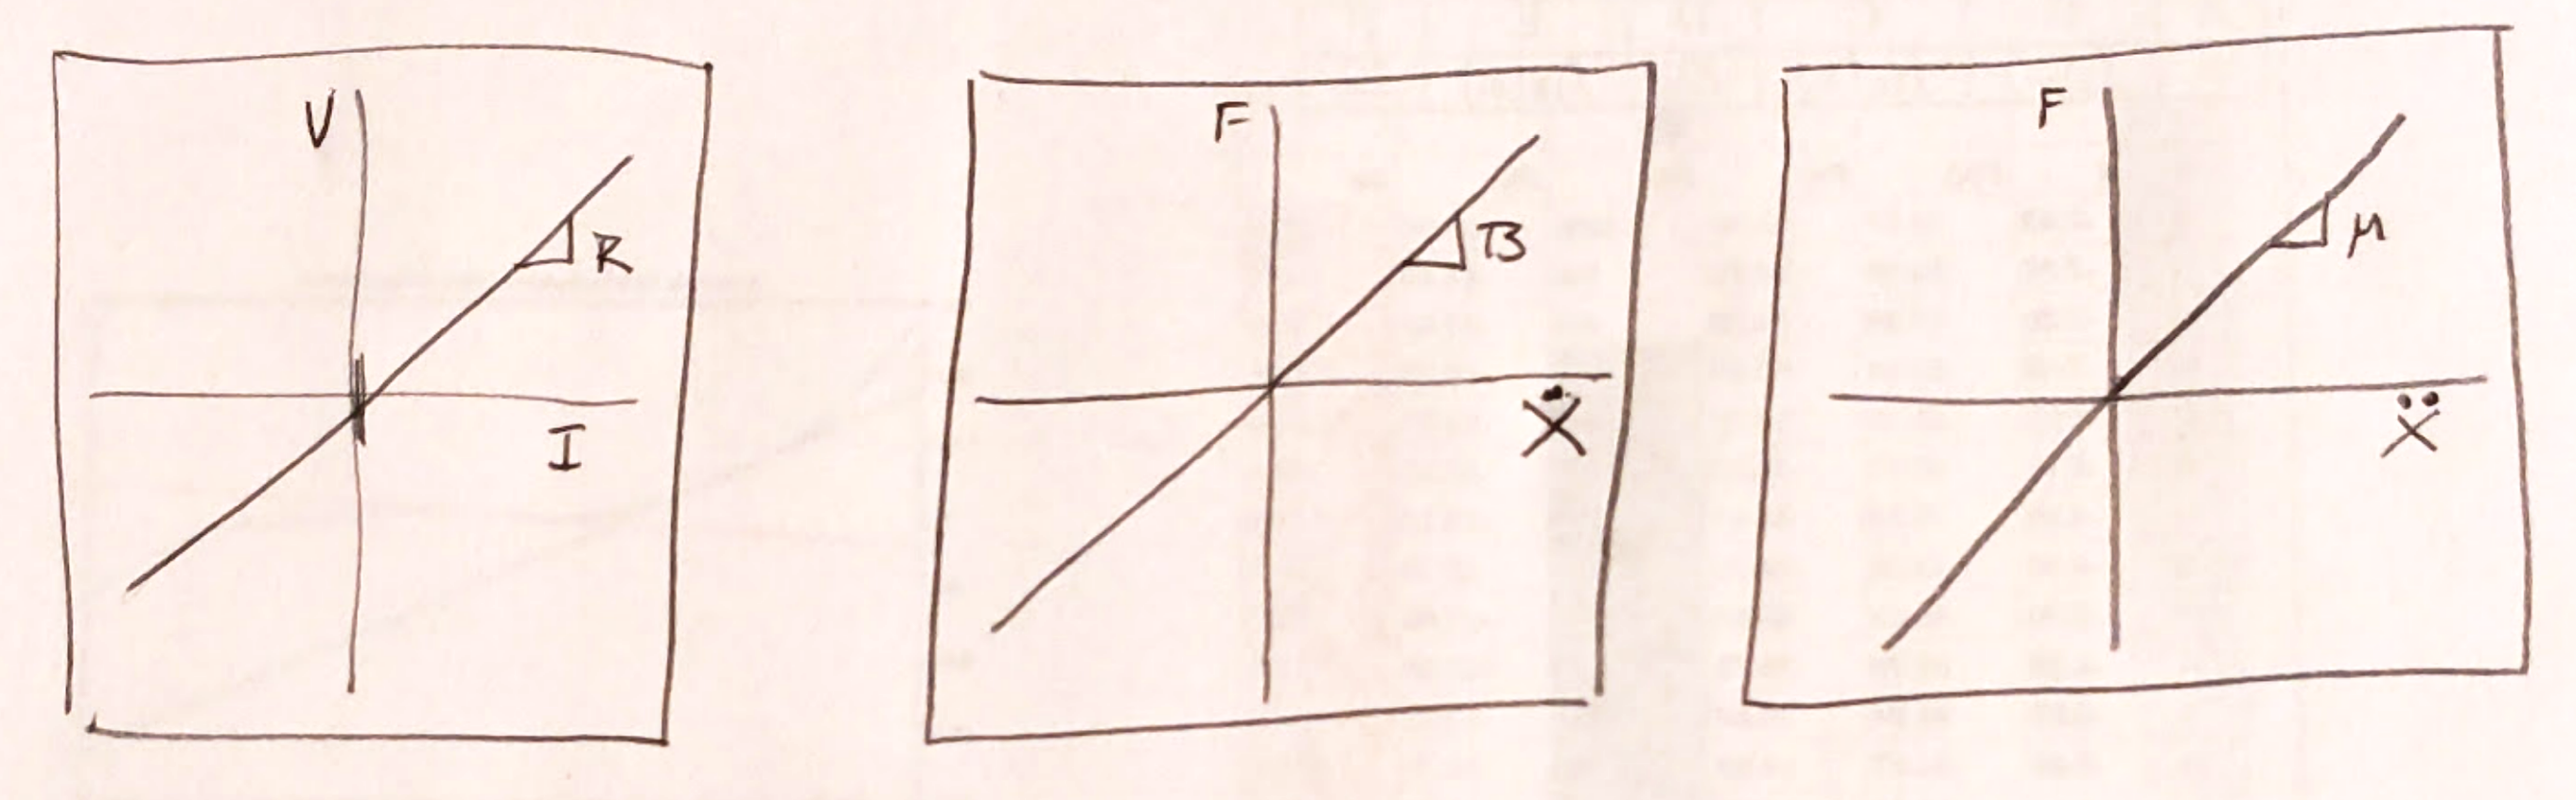
\includegraphics[width=150mm]{figs02/Q68B24.png}



\section{Equations of Motion}

Let's assume a system componsed of multiple masses connected by springs and dampers among each other.   A force $F_i$ acts on each mass, $M_i$.   D'Alembert's Principle equates the famous inertial force $f=m\ddot{x}$ to all the other forces acting on a body.   In a form that we will use:

\bq\label{D'Alembert}
M_i \ddot{x} + \sum_j B_j(\dot{x}_i - \dot{x}_j) + \sum_k K_k(x_i - x_k) = F_i
\eq

where there are several damping components connected between the mass $M_i$ and other masses indicated by $j$, and there are several
spring components connected to some other masses indicated by $k$.  We write this equation for each mass in the system.

Equation \ref{D'Alembert} is refered to as an Equation of Motion (EOM).

$F$ indicates external forces imposed on the mass from sources other than springs and dampers in the system such as an actuator.  If the translational system is vertical, the force of gravity would be one such force, $F=Mg$.

The signs in equations of motion can be tricky.   There is really no ``correct" sign for each term, because the equation is valid if you multiply both sides by $-1$.   However if we stick with the following rules, we can write equations of motion in a consistent way so that we can easily keep signs straight:

\begin{itemize}

  \item The positive term in each subtraction associated with $B$ and $K$ must be the displacement of the mass for which the current EOM is being written.
  \item Keep all position sign conventions consistent.  For example, all displacments positive ``to the right" or positive ``facing up".
  \item Keep the sign convention of the external applied force the same as for the displacements and keep it alone on the right-hand-side.

\end{itemize}






\begin{ExampleSmall}

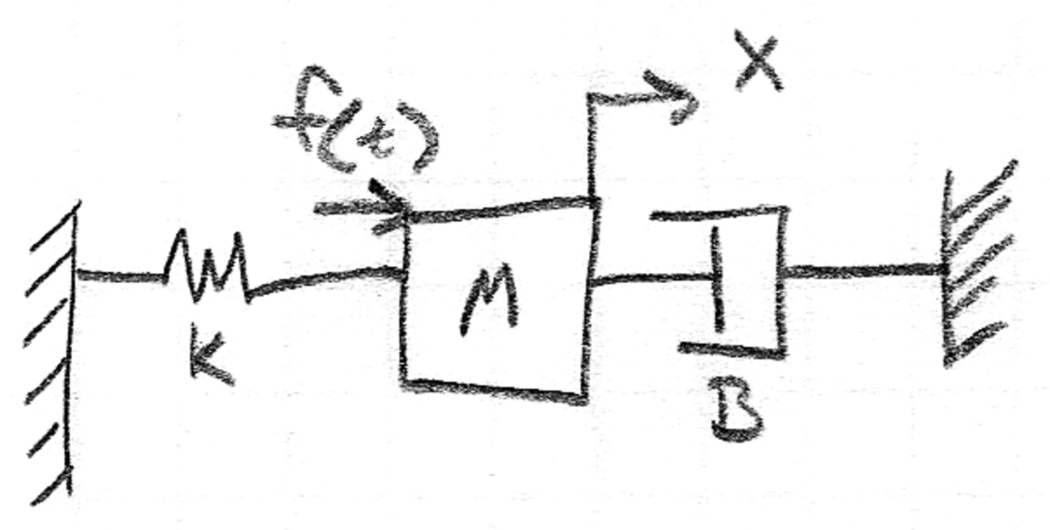
\includegraphics[width=3.0in]{figs02/00721a.png}

writing the EOM for this one mass:

\[
M\ddot{x} + B(\dot{x} - 0) + K(x-0) = f(t)
\]

The spring and damper are each connected to ground.  Ground is a point defined by $x=0$, and $\dot{x}=0$.   Here we have shown $-0$ in the EOM damping and stiffness terms for completeness.
Normally when we have springs and dampers grounded we can skip the subtraction step and the EOM is simply:

\[
M\ddot{x} + B\dot{x} + Kx = f(t)
\]

\end{ExampleSmall}





\begin{ExampleSmall}\label{example2dampers}
Here we have still a single mass, but multiple dampers are connected.   Note that it makes no difference if the ``ground" symbol is located to the left or right of the mass, it still represents $x=0, \dot{x}=0$.



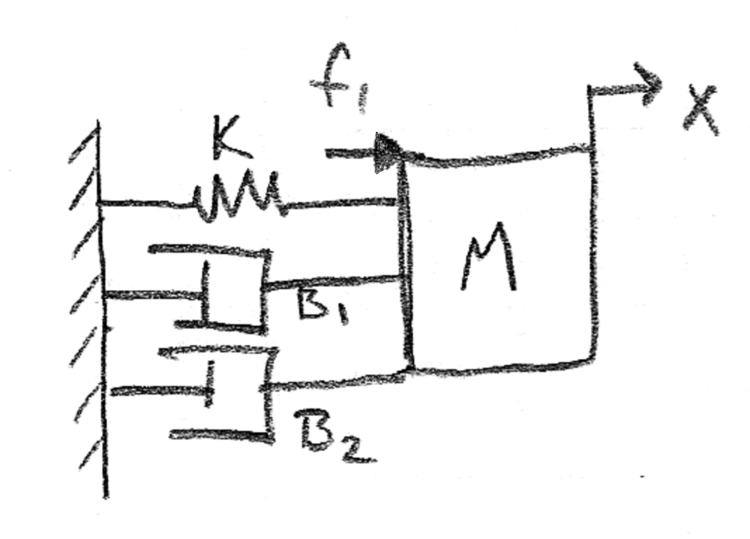
\includegraphics[width=2.5in]{figs02/00722a.png}


EOM:
\[
M\ddot{x} + B_1(\dot{x}-0)+B_2(\dot{x}-0)+K(x-0) = f(t)
\]
Simplifying

\[
M\ddot{x} + (B_1+B_2)\dot{x}+Kx = f(t)
\]
\end{ExampleSmall}


\subsection{Parallel and Series Combinations}
We were able to simplify the EOM in Example \thechapter.\ref{example2dampers} in a way which added the two dampers together.   If you think about a simple modification to Example \thechapter.\ref{example2dampers}, you can see that the same could be done with springs as well.
The general principle is that springs and dampers combine (like capacitors in electric circuits) (Figure \ref{seriessprings}) as follows:

Springs and dampers in {\it parallel} can be combined by addition.

Springs and dampers in {\it series}   can be combined like parallel resistors:

\begin{figure}[h]\centering
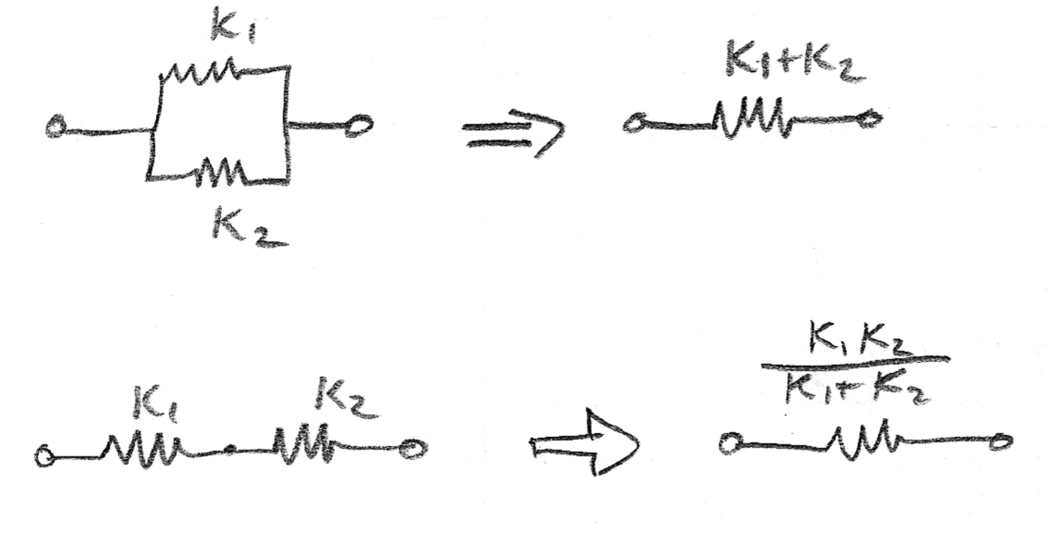
\includegraphics[width=3.5in]{figs02/00723a.png}
\caption{Springs in parallel and series can be combined (like capacitors).}\label{seriessprings}
\end{figure}


\hrule
{\it Proof:}
Consider two springs in series.
The force, $f$ is the same throughout all elements of a serial chain, and both springs independently obey Hooke's Law:

\[
f = K_1\Delta x_1 = K_2\Delta x_2
\]
The total change in length due to the applied force, $f$, is
\[
\Delta x = \Delta x_1 + \Delta x_2
\]

\[
\Delta x = \frac{f}{K_1} + \frac{f}{K_2}
\]

\bq
K_T = \frac{f}{\Delta x} = \frac {1}  {1/K_1 + 1/K_2} = \frac  {K_1K_2} {K_1+K_2}
\eq
\hrule

An almost identical proof can be made for series connected dampers.

However, Mass, $M$ is different (Figure \ref{addtwomasses}) because of the unique property that the force on a mass depends on the acceleration only with respect to the inertial frame:

\[
f = m\ddot{x}, \quad \mathrm{NOT} \quad f = m(\ddot{x}_i - \ddot{x}_j)
\]
Thus


\begin{figure}[h]\centering
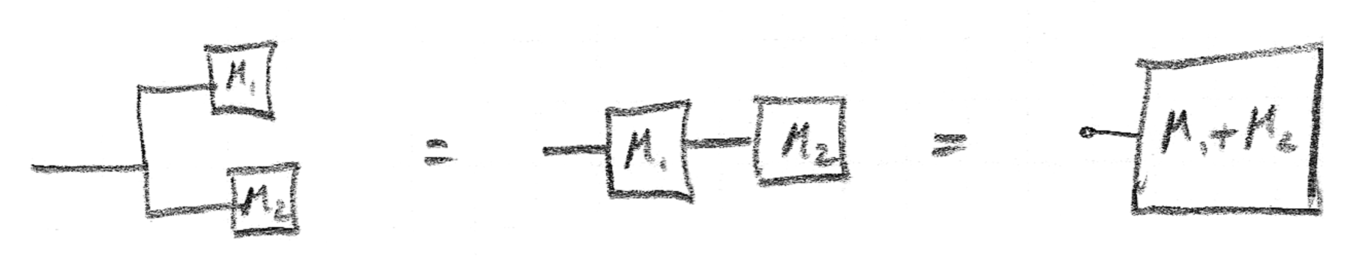
\includegraphics[width=4.5in]{figs02/00724a.png}
\caption{Add two masses which ever way they are combined.}\label{addtwomasses}
\end{figure}

What about the case where a spring and damper are connected in series (Figure \ref{springseriesdamper})?


\begin{figure}\centering
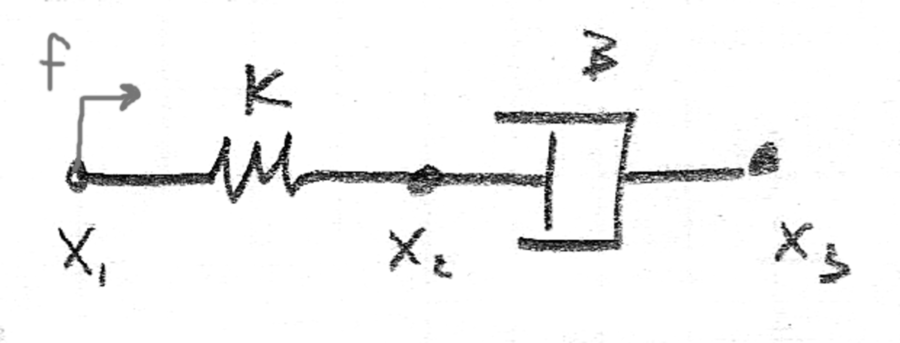
\includegraphics[width=3.0in]{figs02/00725a.png}
\caption{If a spring and damper are connected in series, a new EOM must be constructed for the node in between ($x_2$).}\label{springseriesdamper}
\end{figure}

Using a similar analysis based on the fact that $f$ is the same in both elements of a serial chain:
\[
f = K(x_1-x_2) = B(\dot{x}_2-\dot{x}_3)
\]

The difference here is that we have a new unknown $x_2$.    This new unknown requires a new EOM however $m_2 =0$.   The EOMS for the system of Figure \ref{springseriesdamper} are thus:
\[
K(x_1-x_2) = f
\]
\[
0\ddot{x_2} + K(x_2-x_1) + B(\dot{x}_2-\dot{x}_3) = 0
\]
\[
B(\dot{x}_3-\dot{x}_2) = 0
\]






\subsection{Multiple Masses and EOMs}
When there are multiple independent masses (who's displacements, $x_i$ are not the same) then we need a separate EOM for each mass (Example \thechapter.\ref{MultipleEOMs}).
In a general system with multiple masses, dampers or springs can be connected between any two of the masses.  This is why we used the subscripts and the subtractions in Equation \ref{D'Alembert}.



\begin{ExampleSmall}\label{MultipleEOMs}


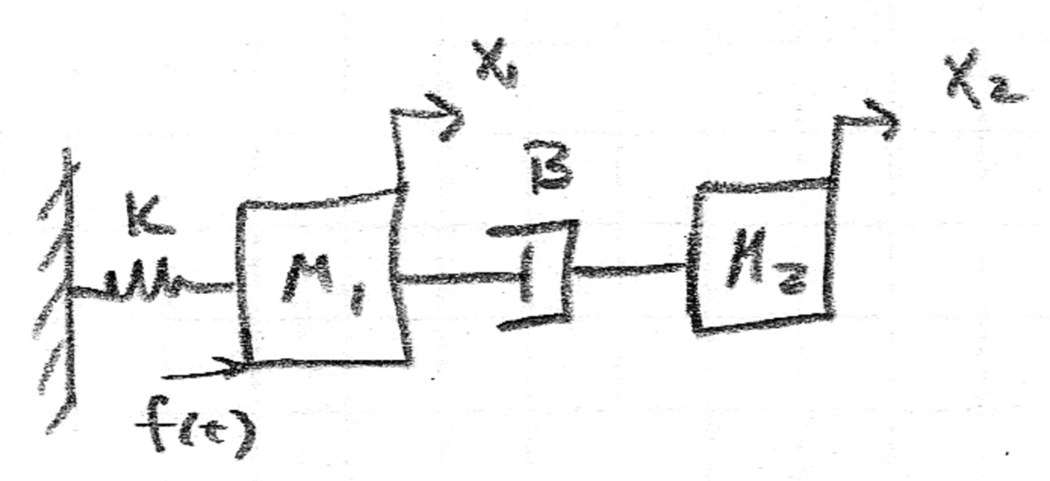
\includegraphics[width=3.5in]{figs02/00726a.png}



By applying Equation \ref{D'Alembert} to each mass,
\[
(M_1) \qquad M_1\ddot{x}_1 + B(\dot{x}_1 - \dot{x}_2) + Kx_1 = f(t)
\]
\[
(M_2) \qquad M_2\ddot{x}_2 + B(\dot{x}_2-\dot{x}_1)  = 0
\]

Note that each EOM for mass $i$ always begins with $M_i\ddot{x}_i$ and that in the $B,K$ terms of EOM$_i$, $x_i$ is always taken positive.
\end{ExampleSmall}





\section{Conversion to Transfer Function}

EOMs are {\it Linear Ordinary Differential Equations}, LODEs.  As such, we can easily apply the Laplace Transform.
Using the EOMs of Example \thechapter.\ref{MultipleEOMs},
\[
M_1X_1(s)s^2 + BX_1(s)s - BX_2(s)s + KX_1(s) = F(s)
\]
\[
M_2X_2(s)s^2 + BX_2(s)s - BX_1(s)s = 0
\]
Note that we have assumed zero initial conditions.   What does this assumption mean?  Mathematically it means
\[
x_i(t=0) = 0, \quad \dot{x}_i(t=0) = 0, \quad \ddot{x}_i(t=0) = 0
\]
and physically this corresponds to the system being at rest and having no kinetic or potential energy.

We will use the Laplace transform to solve for a {\it Transfer Function}.   Transfer functions are ratios between the Laplace Transforms of two physical variables.  Examples:

\[
\frac{X_2(s)}{F(s)} \qquad
\frac{X_1(s)}{X_2(s)} \qquad \mathrm{etc.}
\]

Often we need to analyze a system when we know its input (say $X(s)$) but do not know its output (say $Y(s)$).  If we can obtain the transfer function
\[
G(s) = \frac{Y(s)}{X(s)}
\]

then we can get the Laplace transform of the output by
\[
Y(s) = G(s)X(s)
\]

The transfer function is obtained by algebraically manipulating the Laplace transform of one or more EOMs.
Sometimes multiple EOMs have to be solved simultaneously to get the transfer function.

\begin{ExampleSmall}\label{TransferFunctionExample}
For the system of Example \thechapter.\ref{example2dampers}, let's find the transfer function
\[
G(s) = \frac {X(s)}{F(s)}
\]
Using this transfer function we could compute the displacement as a function of the input force.


There is only one mass and thus only one EOM.  Starting with the EOM

\[
M\ddot{x} + (B_1+B_2)\dot{x}+Kx = f(t)
\]

First take the Laplace Transform:
\[
(LT) \qquad   MX(s)s^2 + (B_1+B_2)X(s)s + KX(s) = F(s)
\]
then we factor out $X(s)$ from each term giving
\[
X(s)\left( Ms^2 +(B_1+B_2)s + K \right) = F(s)
\]
dividing through we get the transfer function
\[
G(s) = \frac {X(s)}{F(s)} = \frac {1}{Ms^2 + (B_1+B_2)s + K }
\]

\end{ExampleSmall}


We will find it useful to {\it normalize} each transfer function before further analysis.   This means that we will manipulate each polynomial in $s$ so that the coefficient of  highest power of $s$ is 1\footnote{Known as a ''monic" polynomial.}.    This is accomplished by just dividing through by the coefficient of the highest power of $s$ as a final step.


\begin{ExampleSmall}
Normalize the transfer function of Example \thechapter.\ref{TransferFunctionExample}.

Dividing through top and bottom by $M$,

\[
G(s) = \frac {X(s)}{F(s)} = \frac {1/M}{s^2 + \frac{B_1+B_2}{M}s + \frac{K}{M} }
\]
\end{ExampleSmall}


\section{Examples}

%%%%%%%%%%%%%%%%%%%%%%%%%%%%%%%%%%%%%%%%%%%%%%%%%%%%%%%%%%%%%%%%%%%%%%%%%%%%%%%%%%%%%%%%%%%%%%%%%%%%%%%%%
\begin{Example}\label{3MassExample}
Two sliding masses.


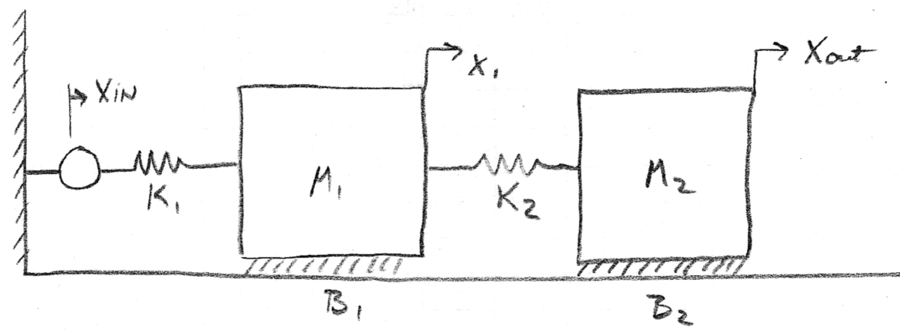
\includegraphics[width=3.0in]{figs02/00727a.png}

(Note that in this diagram, we used hatching between the mass and ground to indicate damping ($B_1, B_2$).  This symbol is commonly used because it visually suggests sliding friction.

Find
\[
G(s) = \frac{X_{out}(s)}{X_{in}(s)}
\]
Normalize the Denominator of the solution.

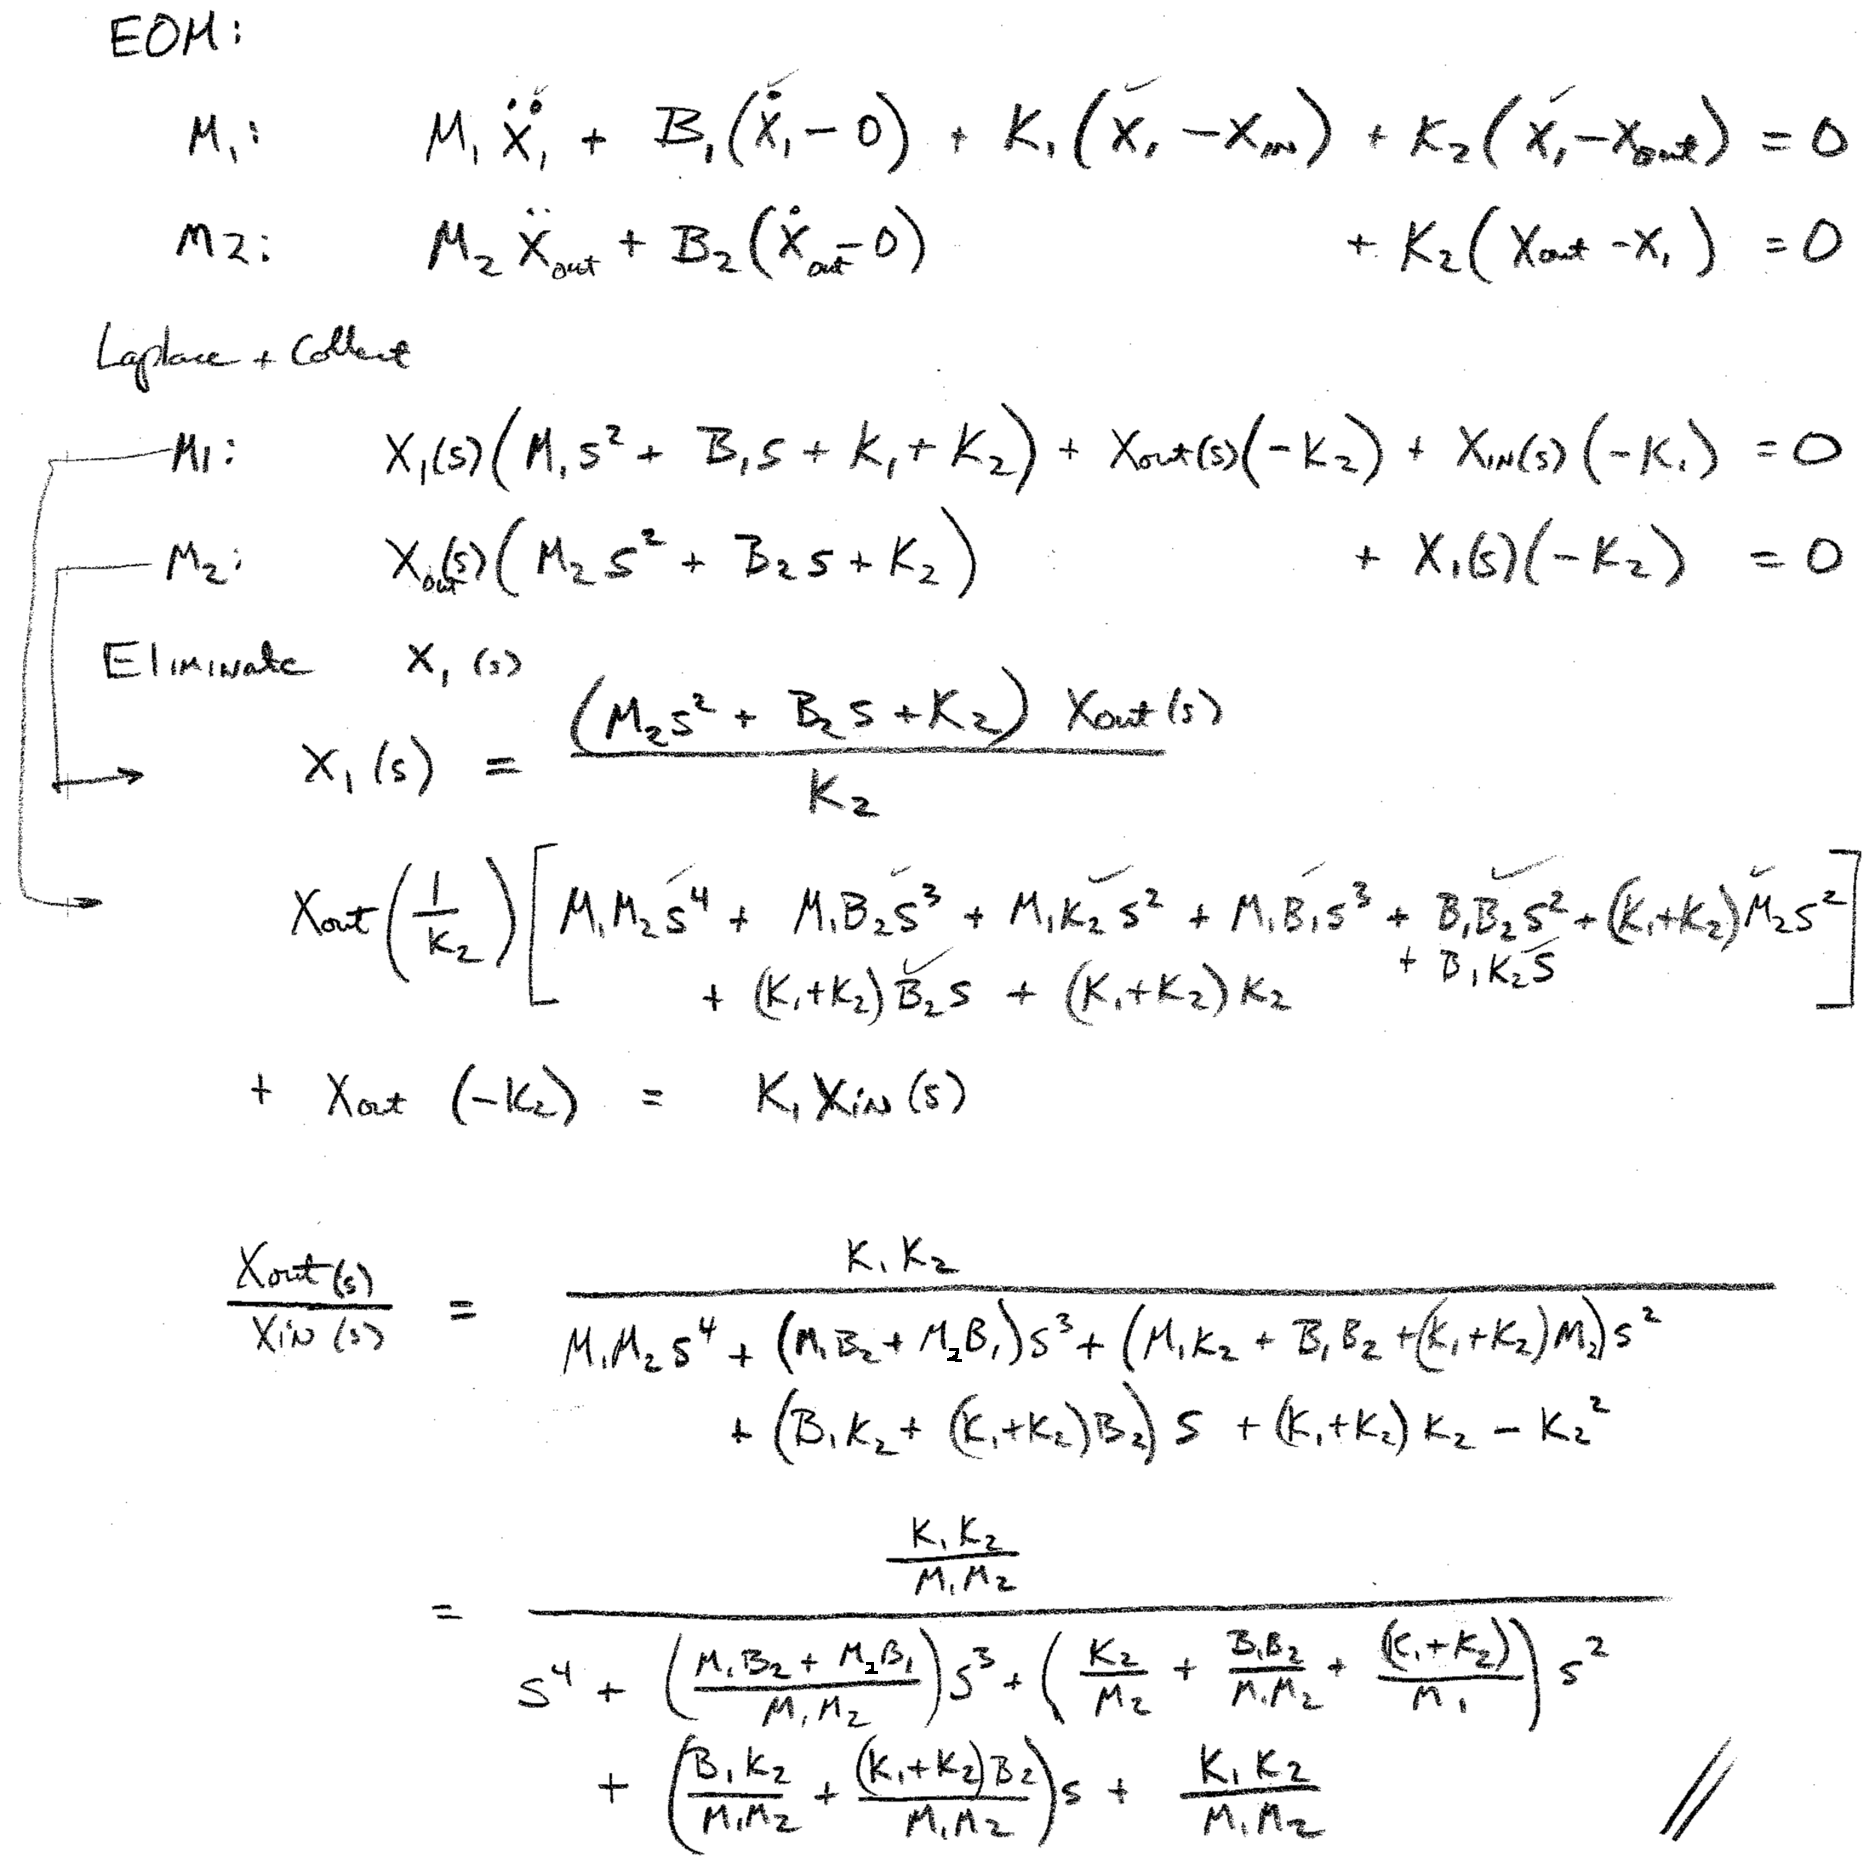
\includegraphics[width=6.25in]{figs02/00729a.png}

\end{Example}



%%%%%%%%%%%%%%%%%%%%%%%%%%%%%%%%%%%%%%%%%%%%%%%%%%%%%%%%%%%%%%%%%%%%%%%%%%%%%%%%%%%%%%%%%%%%%%%%%%%%%%%%%

\begin{Example}\label{ExampleCarSuspensionTF}   %2.8
Car Suspension Example

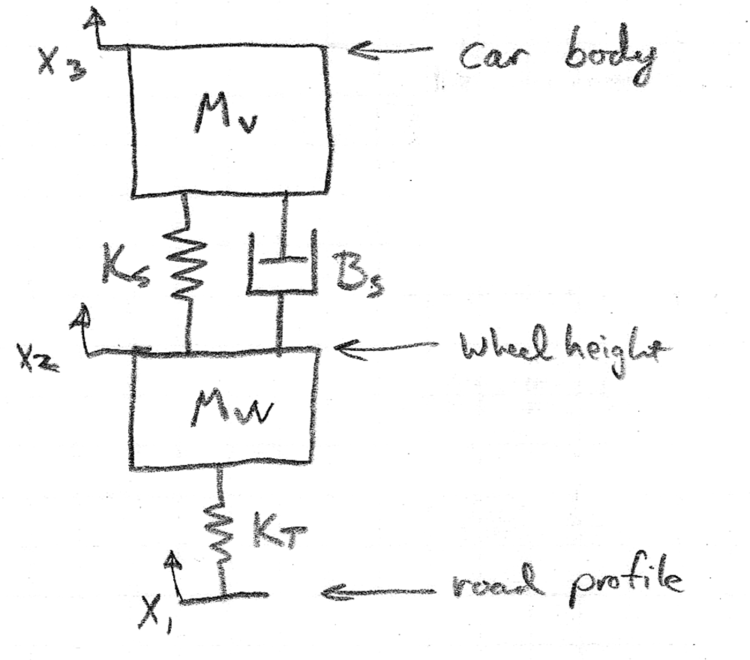
\includegraphics[width=2.5in]{figs02/00730a.png}    Find the transfer function from road ($x_1(s)$) to body ($x_3(s)$).
Normalize the denominator.


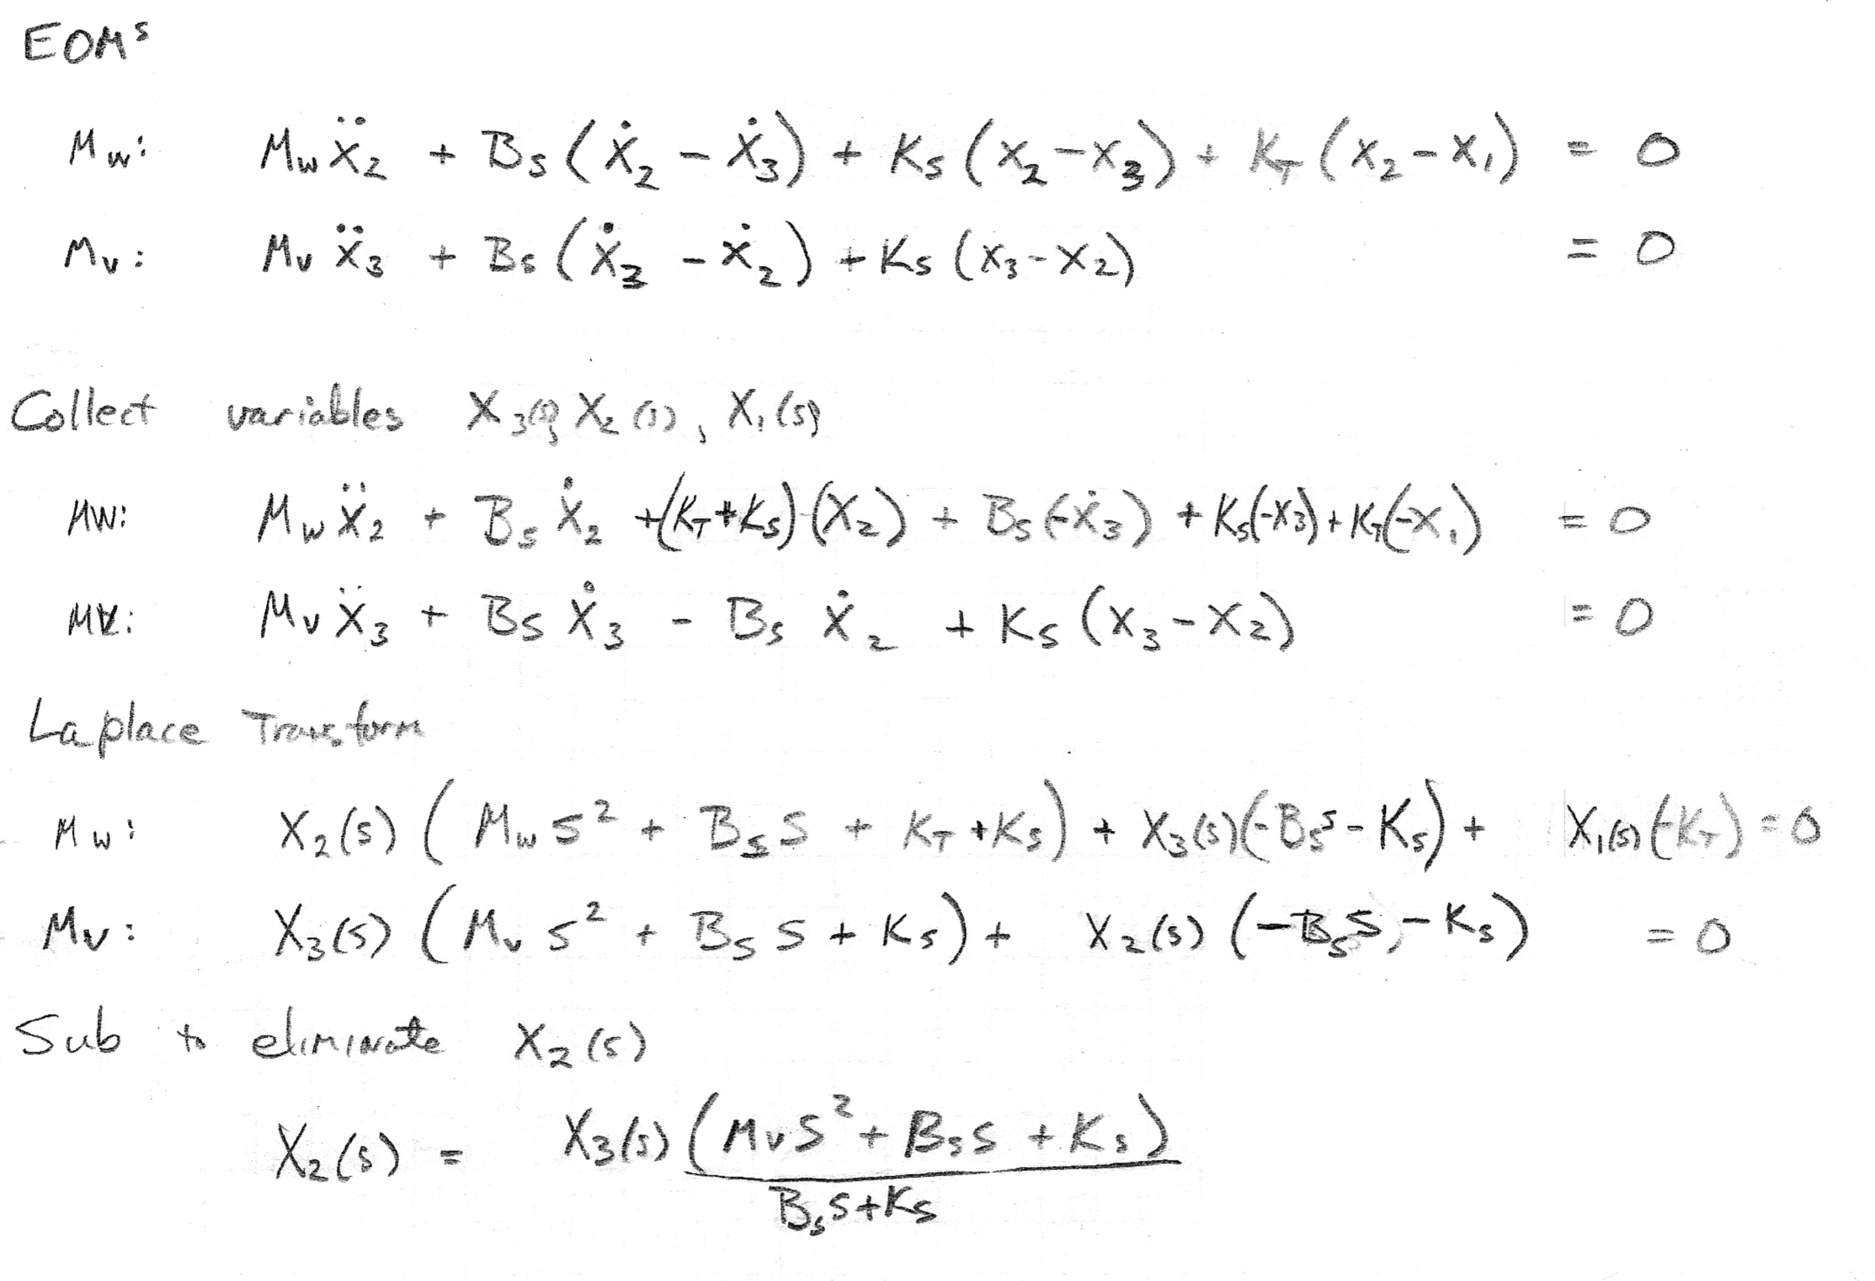
\includegraphics[width=6.25in]{figs02/00731a.png}

\end{Example}

%
\begin{ExampleCont}
  %
Note what we have done under ``Collect Variables" above is to simply collect terms according to the motion variables in a systematic
way.  Specifically we can stay organized by filling
out a table re-arranging the EOMs as follows:\vspace{0.3in}



% Make table rows deeper
\renewcommand\arraystretch{1.5}% Vertical Row size, 1.0 is for standard spacing)


\begin{tabular}{|p{0.35in}|p{0.55in}|p{0.55in}|p{0.55in}|p{0.35in}|p{0.65in}|p{0.55in}|p{0.55in}|p{0.35in}|}\hline
  Eqn\# & $\ddot{x_j}$ & $\dot{x_1}$ & $x_1$  & $\dot{x_2}$ & ${x_2} $& $\dot{x_3}$ & ${x_3} $ &  = \\ \hline
  (1)   & $M_w\ddot{x}_2$ & 0 & $(-K_T)$ & $B_S$    & $(K_T+K_S)$ & $(-B_S)$ & $(-K_S)$ & 0  \\ \hline
  (2)   & $M_v\ddot{x}_3$ & 0 & 0        & $(-B_S)$ & $(-K_S)$    & $B_S$    & $K_S$    & 0 \\ \hline
\end{tabular}

Note that our system equations seem to lack an input (which would be on the right-hand-side i.e. the
last column of our tabular form).  Thinking back to cars, the input would be changes in road height,
$x_1$ (which is not attached to a mass).  We can thus re-do the table to move $x_1$ terms to
the right hand side:

\begin{tabular}{|p{0.35in}|p{0.55in}|p{0.55in}|p{0.55in}|p{0.35in}|p{0.65in}|p{0.55in}|p{0.55in}|p{0.35in}|}\hline
  Eqn\# & $\ddot{x_j}$ & $\dot{x_1}$ & $x_1$  & $\dot{x_2}$ & ${x_2} $& $\dot{x_3}$ & ${x_3} $ &  = \\ \hline
  (1)   & $M_w\ddot{x}_2$ & 0 & $0$ & $B_S$    & $(K_T+K_S)$ & $(-B_S)$ & $(-K_S)$ & $K_Tx_1$ \\ \hline
  (2)   & $M_v\ddot{x}_3$ & 0 & 0        & $(-B_S)$ & $(-K_S)$    & $B_S$    & $K_S$    & 0 \\ \hline
\end{tabular}
This tabular method will be useful later when we derive state space system equations.

Getting back to the transfer function:

%  \includegraphics[width=6.25in]{figs02/00961a.png}
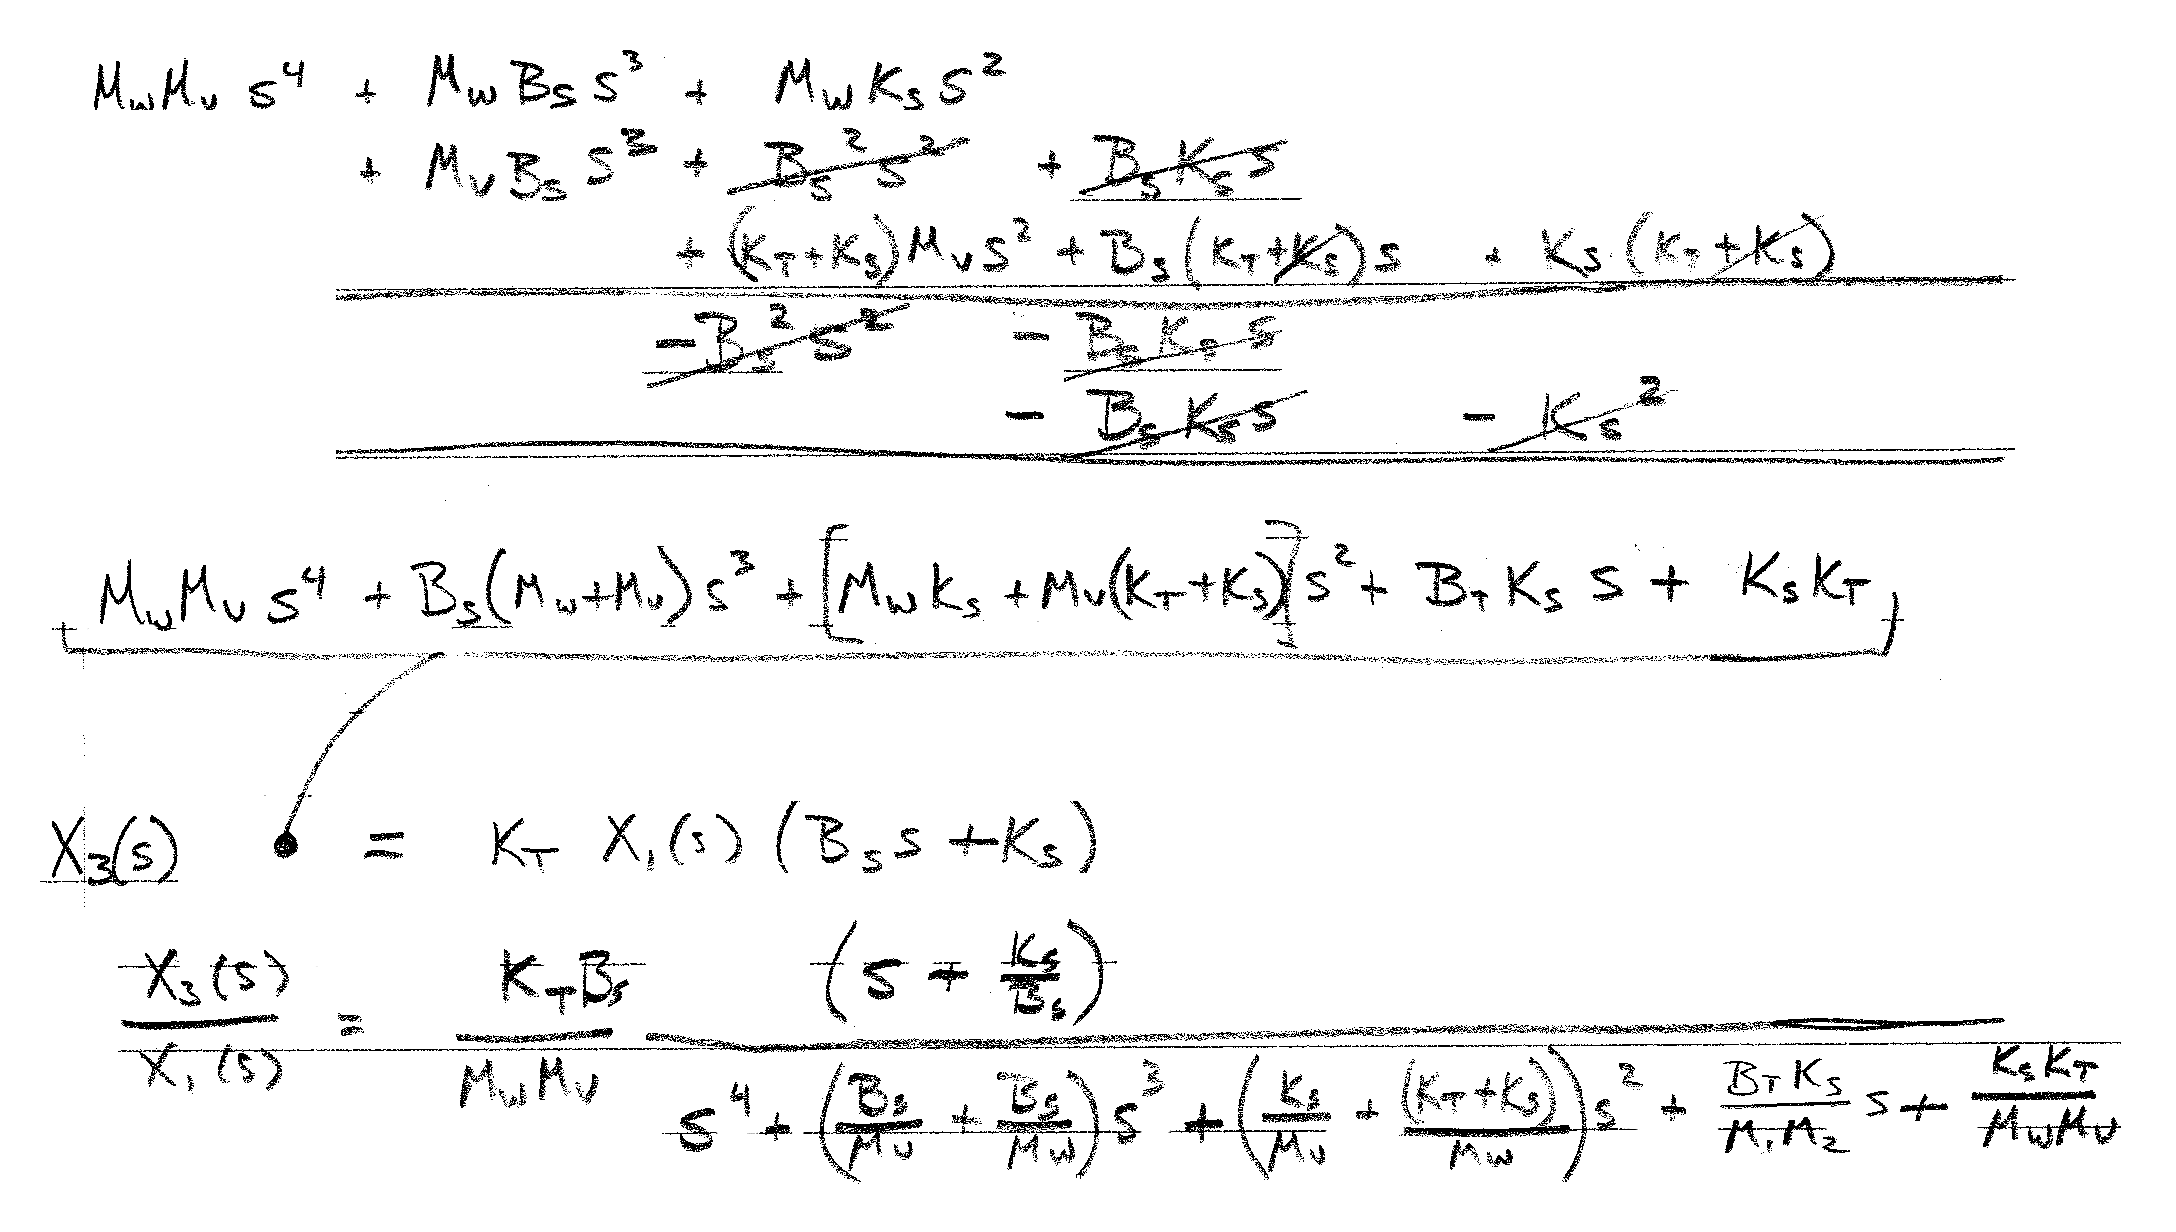
\includegraphics[width=6.0in]{figs02/00961.png}

\end{ExampleCont}



\section{Finding Errors through Dimensional Analysis}

Once the numerator and denominator of the transfer function are normalized, we can exploit dimensional analysis to check our work for errors.   We rely on the fact that for quantities to be added together they must have the same units.  What are the units of $s$?

$s$ represents frequency and so has the units of inverse seconds, $\mathrm{sec}^{-1}$.  Also each physical parameter has units.  The MKS system has only three {\it fundamental units}, meters, kg, and seconds. Assuming the MKS system, each physical parameter has the units given in Table \ref{unitstable}.

\begin{table}[h]\centering
\renewcommand{\arraystretch}{1.5} %<- modify value to suit your needs
\begin{tabular}{c|l||c|l}
Name	& Fundamental Units & Name	& Fundamental Units \\ \hline
$s$	& $\mathrm{sec}^{-1}$      & $B$	& $\frac{kg}{\mathrm{sec}}$  \\
$s^n$   & $\mathrm{sec}^{-n}$  & $K$	& $\frac{kg}{\mathrm{sec}^2}$  \\
& & $M$	& $kg$ \\
\end{tabular}
\caption{Fundamental MKS units for $s$ and the physical parameters.}\label{unitstable}
\end{table}

Now suppose the denominator of a transfer function has been normalized and then begins with $s^4$.   Then through dimensional analysis, we know that all the subsequent terms in the polynomial must have the same units, namely sec$^{-4}$.  This can often be an easy way to find an error in the transfer function without checking each step. Note that you can also apply this to the tabular version of
Example 2.\ref{ExampleCarSuspensionTF}
by making sure all entries in each column have the same units.




\begin{Example}\label{DimensionalAnalysisExample}

We have derived the following transfer function:

\[
G(s) = \left( \frac {B} {M_1M_2}\right) \frac{s+K/M}
 {s^4 + \frac{M_1+M_2}{M_1M_2}Bs^3+(1/M_1+1/M_2)2BKs^2+\frac{2BK}{M_1M_2}s+\frac{3K^2}{M_1M_2}}
\]

Check for errors using dimensional analysis:
We  ignore the normalizing term $\frac{B}{M_1M_2}$ because it is outside the additions.  It could be right or wrong, but
dimensional analysis won't help us with this particular term.


{\bf Numerator:}
\[
s+K/M
\]
First, we have $s$.  The units of $s$ are sec$^{-1}$.  Checking the next term $\frac{K}{M}$, we convert each term into its fundamental units and multiply them:

\begin{tabular}{c|c|c}
$K$ 	&	$1/M$  &	\\ \hline
$\frac{kg}{\mathrm{sec}^2}$ & $1/kg$ & $= \frac{1}{\mathrm{sec}^2} \neq \mathrm{sec}^{-1}$ \\
\end{tabular}

The units do not agree with sec$^{-1}$ so this is an \hspace{0.25in}  {\bf ERROR!}


\vspace{0.15in}

{\bf Denominator: }
\vspace{0.2in}
The first term is $s^4$.  Therefore, all terms in demoninator must have net units of $\mathrm{sec}^{-4}$.  The next term is
\[
\frac{M_1+M_2}{M_1M_2}Bs^3
\]
In the $\frac{M_1+M_2}{M_1M_2}$ term, the units reduce to $1/M$ by cancellation.   Therefore we can break it down as

\begin{tabular}{c|c|c|c}
$1/M$	& $B$      & $s^3$ & \\ \hline
$1/kg$  & $kg/sec$ & $\mathrm{sec}^{-3}$ & $= \mathrm{sec}^{-4}$
\end{tabular}
\hspace{0.25in}  {\bf CORRECT}



Continuing in this manner:
\[
(1/M_1+1/M_2)2BKs^2
\]

\begin{tabular}{c|c|c|c|c}
$1/M$	& $2B$	& $K$	& $s^2$ & \\ \hline
$1/kg$  & $kg/\mathrm{sec}$	& $kg/\mathrm{sec}^2$	& $1/\mathrm{sec}^2$	& $= \frac{kg}{\mathrm{sec}^5} \neq \mathrm{sec}^{-4}$
\end{tabular}
\hspace{0.25in}{\bf ERROR!}


\[
\frac{2BK}{M_1M_2}s
\]


\begin{tabular}{c|c|c|c|c}
$1/M^2$	  & $2B$		& $K$	& $s$ & \\ \hline
$1/kg^2$  & $kg/\mathrm{sec}$	& $kg/\mathrm{sec}^2$	& $1/\mathrm{sec}$	& $= \frac{1}{\mathrm{sec}^4} = \mathrm{sec}^{-4}$
\end{tabular}
\hspace{0.25in}  {\bf CORRECT}



\[
\frac{3K^2}{M_1M_2}
\]

\begin{tabular}{c|c|c}
$1/M^2$	& $3K^2$   & \\ \hline
$1/kg^2$  & $kg^2/\mathrm{sec}^4$	& $= \frac{1}{\mathrm{sec}^4} = \mathrm{sec}^{-4}$
\end{tabular}\hspace{0.25in}  {\bf CORRECT}

\end{Example}

\section{More complex problems}
The structure we have added to the EOMs in Example 2.\ref{ExampleCarSuspensionTF}, as well as the
use of dimensional analysis for easy debugging of your equations, makes it easier than you
might expect to analyze a more complex system (or break a system down into a more detailed model).
For example, let's write down equations of motion for a kind of intimidating
system with 4 masses and many springs and
dampers as in Figure \ref{complexDynSystem}.


\begin{figure}\centering
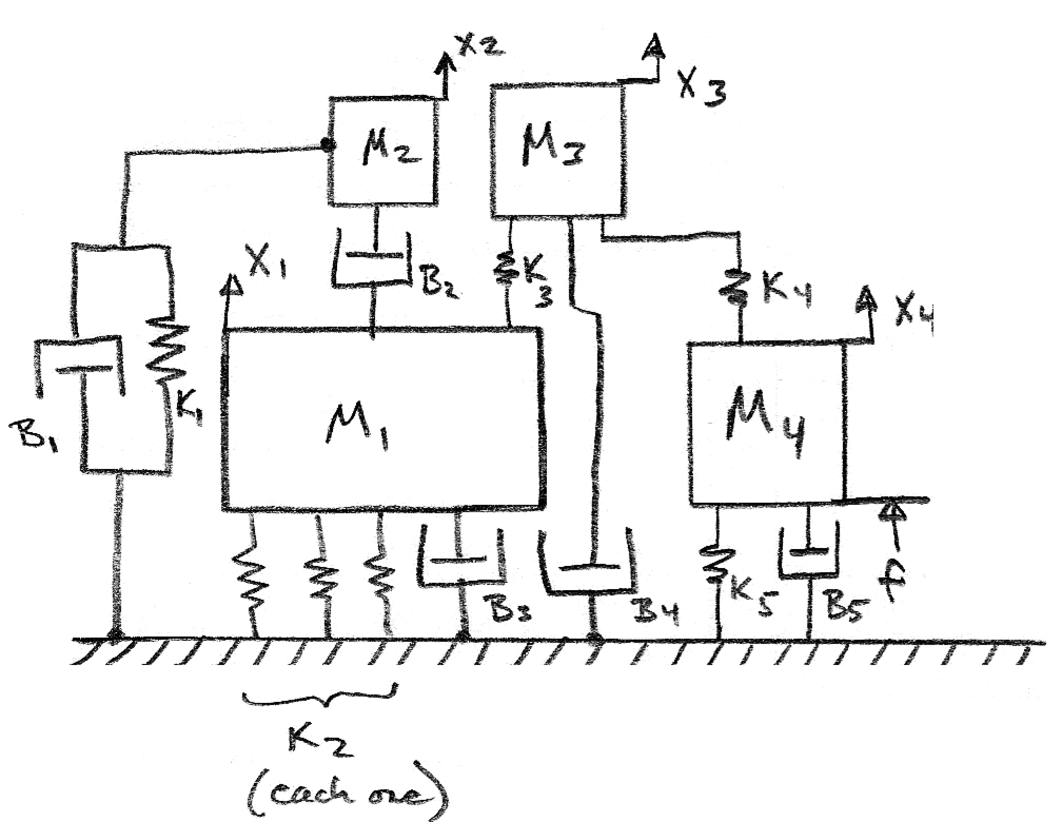
\includegraphics[width=90mm]{figs02/00933a.png}
\caption{A system with 4 masses and numerous springs and dampers connecting them.}
\label{complexDynSystem}
\end{figure}

\begin{Example}
  Write the 4 EOMs for the system of Figure \ref{complexDynSystem}.

Summing forces on each mass:
\[
M_1\ddot{x}_1 + B_3\dot{x}_1+B_2(\dot{x}_1-\dot{x}_2) +3K_2x_1+K_3(x_1-x_3)  = 0
\]
\[
M_2\ddot{x}_2 + B_2(\dot{x}_2-\dot{x}_1)+B_1\dot{x}_2+K_1x_2 = 0
\]
\[
M_3\ddot{x}_3 + B_4\dot{x}_3+K_3(x_3-x_1)+K_4(x_3-x_4)=0
\]
\[
M_4\ddot{x}_4+B_5\dot{x}_4+K_4(x_4-x_3)+k_5x_4 = f(t)
\]


Now re-organize the equations into tabular form as above (but changing to a vertical table).   Each equation (column) is a sum and each row is the coefficient of
each variable in the first column.

\begin{tabular}{|c|c|c|c|c|c|}\hline
  Var           & EOM1 & EOM2 & EOM3 & EOM4\\\hline
  $M_j\ddot{x}_j$  & $M_1\ddot{x}_1$&$M_2\ddot{x}_2$&$M_3\ddot{x}_3$ &$M_4\ddot{x}_4$ \\ \hline
  $\dot{x}_1$   & $(B_2+B_3)$ &$(-B_2)$  & 0           & 0 \\ \hline
        $x_1$   & $(3K_2+K3)$ &0         & 0           & 0 \\ \hline
  $\dot{x}_2$   & $-B_2$      & $B_2$    & 0           & 0 \\ \hline
        $x_2$   & 0           & $K_1$    & 0           & 0 \\ \hline
  $\dot{x}_3$   & 0           & 0        & $B_3$       & 0 \\ \hline
        $x_3$   & $(-K_3)$    & 0        & $(K_3+K_4)$ & $(-K_4)$ \\ \hline
  $\dot{x}_4$   & 0           & 0        & 0           & $B_5$    \\ \hline
        $x_4$   & 0           & 0        & $(-K_4)$    & $(K_4+K_5)$ \\ \hline\hline
        =       & 0  & 0  & 0 & $f(t)$ \\ \hline
\end{tabular}


Remember, each vertical column is an equation.  the last line is the right
hand side and the first 9 lines are added to form the right hand side.
Taking the first column as an example:
\[
M_1\ddot{x}_1+(B_2+B_3)\dot{x}_1+(3K_2+K_3)x_1-B_2\dot{x}_2 -K_3x_3 = 0
\]

\end{Example}

Although it is sometimes possible to derive useful transfer functions from
this point, systems of this complexity have many possible transfer functions
(based on selecting different input and output points).
Arranging a complex
system into tabular form like this makes it simple to transition to
the matrix-based State Space form which we will introduce in Chapter
\ref{BasicsStateSpaceChapter}.

Also, let's check our work.   First, since each equation is 2nd order
and $\dot{x} \to sX(s), \; x \to X(s)$, then each row must have the same
units in cols 2-5.   Also all the ``dot'' rows must have $B$ units
and all the $x_j$ rows must have $K$ units.   By these rules  our work
above checks out (but remember, it still could contain some errors!).

Finally,  we used the column form here
to fit on the page but the row form (as in Example
2.\ref{ExampleCarSuspensionTF}) will be a closer match to the matrix equations
we will use.
